% LectureTemplate for ME3050 -  Dynamics Modeling and Controls - Tennessee Technological University
% Tristan Hill - Spring 2020 - Summer 2020 - Fall 2022
% Dynamics Modeling and Controls
% Lecture Module - ODE review - Topic 3  - Trial Solution

% Document settings

%\documentclass{beamer}                  % for presentation ?
\documentclass[handout]{beamer}  % for handout ?

\usepackage{/home/thill/Documents/lectures/dmc_lectures/dmc_lectures}

\newcommand{\TNUM}{3\hspace{2mm}} % Topic number 
\newcommand{\moduletitle}{ODE Review} % Titles and Stuff
\newcommand{\topictitle}{The Trial Solution Method} 

\newcommand{\sectiontitleI}{Exponential Assumption} % More Titles and Stuff
\newcommand{\sectiontitleII}{Complementary Solution}
\newcommand{\sectiontitleIII}{Particular Solution}
\newcommand{\sectiontitleIV}{Apply Initial Conditions}
\newcommand{\sectiontitleV}{Summary - 3 Cases}

\author{ME3050 - Dynamic Modeling and Controls}
\title{Lecture Module - \moduletitle}
\date{Mechanical Engineering\vspc Tennessee Technological University}

\begin{document}
	
	\lstset{language=MATLAB,basicstyle=\ttfamily\small,showstringspaces=false}
	
	\frame{\titlepage \center\begin{framed}\Large \textbf{Topic \TNUM - \topictitle}\end{framed} \vspace{5mm}}
	
	% Section 0 - Outline
	\frame{
		
		\large \textbf{Topic \TNUM - \topictitle} \vspace{3mm}\\
		
		\begin{itemize}
			
			\item \sectiontitleI    \vspc % Section I
			\item \sectiontitleII 	\vspc % Section II
			\item \sectiontitleIII 	\vspc %Section III
			\item \sectiontitleIV 	\vspc %Section IV
			
		\end{itemize}
		
	}
	
	\section{Review}

% Section I
\section{\sectiontitleI}

	% Section I - Frame I
	\frame{ \small
		\frametitle{\sectiontitleI}

\frametitle{Trial Solution Method}
Use the {\bf trial solution method} to solve the ODE. \vspace{2mm}\\
This is an {\bf analytical} method that you learned in calculus but it may have been called something different. In the Zill book it is called {\it Homogenous Linear ... Constant Coefficients (4.3-4.4)}. \vspcc

\[a_2y''+a_1y'+a_0y=f(x)\] 


	}
	
	% Section I - Frame II
	\frame{
		\frametitle{\sectiontitleI}

				    

	}

% Section II
\section{\sectiontitleII}
	
	% Section II - Frame I
	\frame{ \small
		\frametitle{\sectiontitleII}

\underline{Step 1} - Find the {\bf complementary part} of the solution from the \vspace{1mm}\\ left hand side of the ODE alone (LHS=0). \\

\[a_2y''+a_1y'+a_0y=f \hspace{5mm}\rightarrow\hspace{5mm} a_2y''+a_1y'+a_0y=0\] 

Assume an exponential solution for the complementary part. \[y_{complementary}=y_c(x)=\] 

Substitute this solution into the ODE (LHS=0).
	}
		
	% Section II - Frame II
	\frame{ 
		\frametitle{\sectiontitleII}
	
	}



% Section III
\section{\sectiontitleIII}
	
	% Section III - Frame I
	\frame{ \small
		\frametitle{\sectiontitleIII}

\underline{Step 2} - Find the {\bf particular part} of the solution from the entire equation (LHS=RHS). \vspcc  
\[a_2y''+a_1y'+a_0y=f\] 

The {\it form of the particular part} follows the RHS of  the ODE. \vspc

\[y_{particular}=y_p(x)=\]  

Substitute this solution into the ODE above and solve for any unknown constants in $ y_p(x) $. 
		}
		
		% Section III - Frame II
	\frame{ 
		\frametitle{\sectiontitleIII}
	
	}

		
% Section IV:
\section{\sectiontitleIV}

	% Section IV - Frame I
	\frame{ \small
		\frametitle{\sectiontitleIV}

\underline{Step 3} - Now combine the {\bf complementary} and {\bf particular} solutions through {\it superposition}. \\

\[y(x)=y_c(x)+y_p(x)=\] 

The ODE is first order and we have \underline{\hspace{10mm}} unknown. Coincidence?\vspcc

\[y(x)=\]  

This {\bf initial value problem} requires \underline{\hspace{10mm}} intial condition.\vspace{2mm}\\

	}

	% Section IV - Frame II
	\frame{ \small
		\frametitle{\sectiontitleIV}
	

\[y(x=0)=\] 
\[y'(x=0)=\] 

\vspace{40mm}

}
	% Section IV - Frame II
	\frame{ \small
		\frametitle{\sectiontitleIV}
	What does the solution look like this time?\\

\[y(x)=\] 

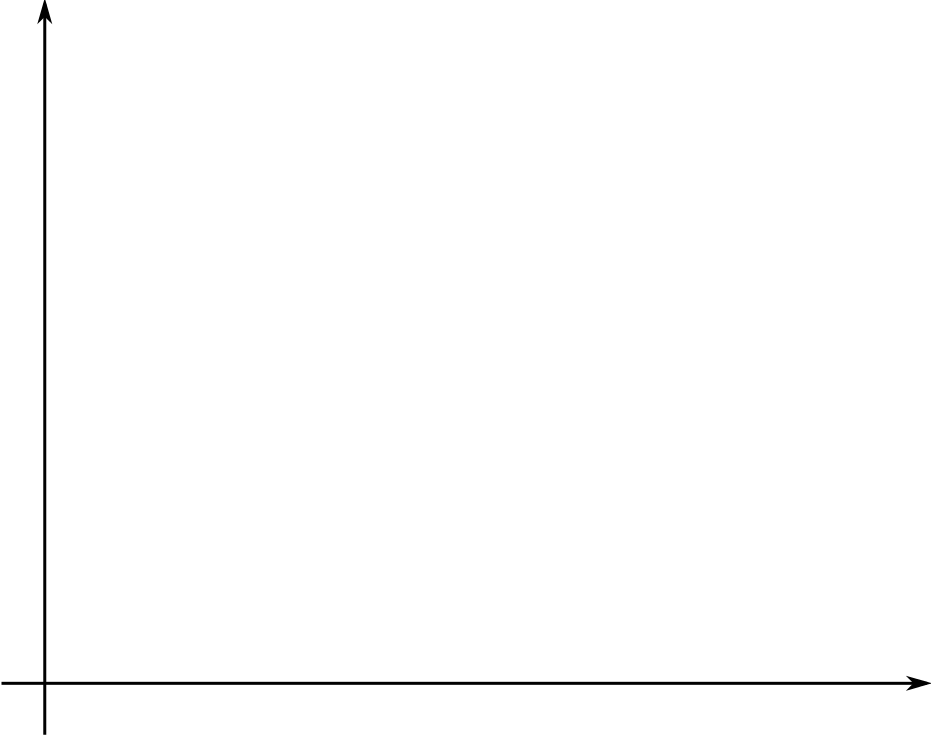
\includegraphics[scale=0.15]{lecture1_fig2.png}\hspace{5mm} 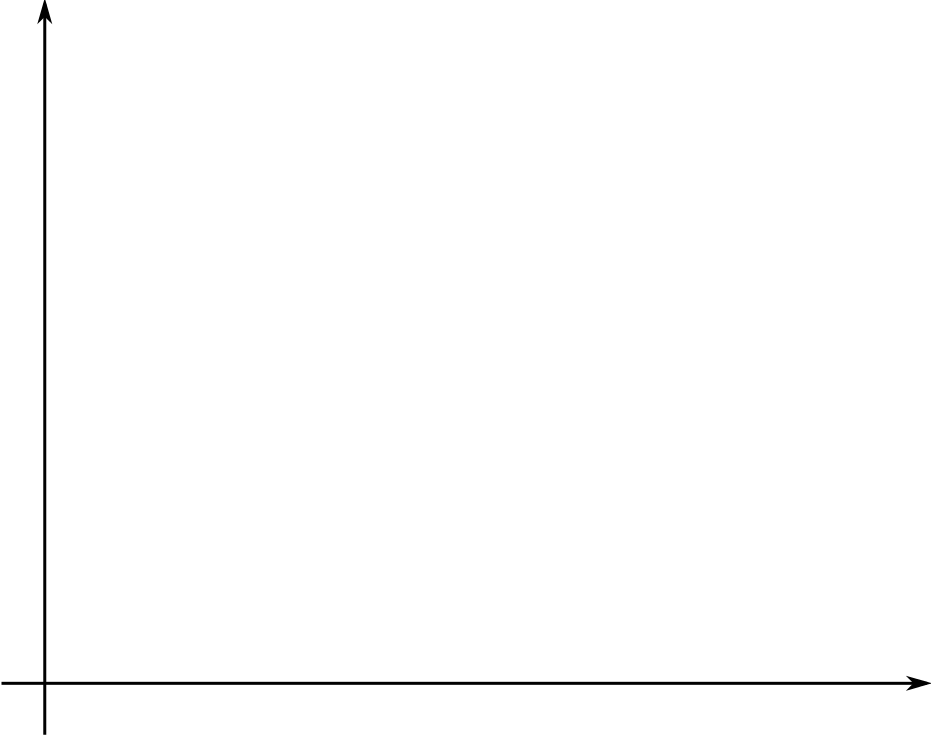
\includegraphics[scale=0.15]{lecture1_fig2.png}
}

	% Section V - Frame I
\frame{ \small
	\frametitle{\sectiontitleV}
	If the differential equation is first and linear, the complementary solution takes the following form. \\

	\[y(x)=Ae^{sx}\] 

	}

	% Section V - Frame II
\frame{ \small
	\frametitle{\sectiontitleV}
	If the differential equation is second order and linear, the {\bf complementary solution } takes one of the following forms. \vspace{2mm}\\

	Case 1: $s_1,s_2\in\mathbb{R} \hspc,\hspc s_1\neq s_2$ 
	\[y(x)=c_1e^{s_1x}+c_2e^{s_2x}\] \vspace{2mm}
	Case 2: $s_1,s_2\in\mathbb{R} \hspc,\hspc s_1=s_2=s$
	\[y(x)=c_1e^{sx}+c_2xe^{sx}\] \vspace{2mm}
	Case 3: $s_1,s_2\notin\mathbb{R} \hspc,\hspc s_1,s_2 = \alpha\pm\beta$
	\[y(x)=e^{\alpha x}\left(c_1 cos\left(\beta x\right)+c_2 sin\left(\beta x\right) \right)\]

}

	% Section V - Frame III
\frame{ \small
	\frametitle{\sectiontitleV}
	The {\bf particular solution} takes the form of the right hand side of the equation. \vspace{2mm}\\ 
	\renewcommand{\arraystretch}{1.5}
	\begin{tabular}{|c|c|c|}
		
		Example & Form & Particular Solution \\ \hline
		
		$... = 10$   & Constant & $y_p=B$ \\
		$... = 12x$  & Linear   & $y_p=Bx+C$\\
		$... = 20e^{2x} $ & Exponential & $y_p=Be^{2x}$ \\
		$... = a cos\left(\beta x\right)$& Sinusoidal &$ Bcos\left(\beta x\right)+Csin\left(\beta x\right)$ \\
		$... = a sin\left(\beta x\right)$& Sinusoidal &$ Bcos\left(\beta x\right)+Csin\left(\beta x\right)$ \\
		
	\end{tabular}

	
}


\end{document}
